The research performed in the paper \emph{MetaFormer is Actually What You Need for Vision} \cite{metaformerPaper} has been very influential in advertising the potential of the \emph{transformer architecture}.
Previously, the model's huge performance was attributed to the attention module, that was introduced in the previous \autoref{sec:architectures-attention}. 
By building alternative models - that shared the structure of the transformer in everything but the attention module - the researchers were able to show that the credit belongs to the structural architecture.

A new class of models, dubbed \emph{metaformer} by the authors, was introduced. 
The architecture's good performance can be motivated through its inductive biases, which will be addressed in \autoref{sec:architectures-biasesmetaformer}.
The following section is only supposed to introduce the naming scheme that is going to be used in the later parts of this thesis.

The general structure of the metaformer can be seen in \autoref{fig:metaformer-architecture}.

\begin{figure}[htbp]
    \centering
    \makebox[\textwidth][c]{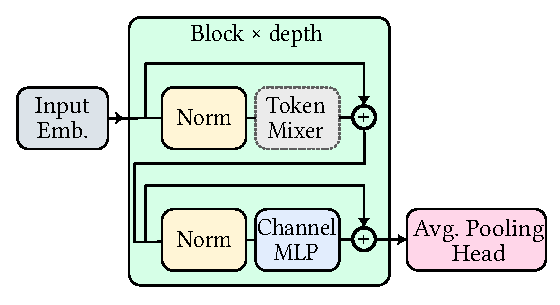
\includegraphics[width=0.8\textwidth]{./architectures/theory/metaformer/metaformer.pdf}}
    \caption{Schematic representation of the \emph{metaformer} concept architecture, adapted to represent the models used in the thesis. 
    The model starts with an input embedding block, that converts the input data into the shape required for the metaformer ($n\times e$) \cite{imageWorth16x16}. This is also the place where possible position encodings are added. 
    After that, the information is passed through \emph{depth} blocks sequentially. 
    A block consists of \emph{norm}, \emph{token mixer}, \emph{residual connection} (+), 
    \emph{norm}, \emph{channel mlp}, \emph{residual connection} (+).
    The model's internal state is brought to the desired output dimension with an \emph{average pooling} operation to get from $n \times e$ to $1 \times e$ and a mlp to get to the desired output dimension $1 \times d_\mathrm{out}$.
    }
    \label{fig:metaformer-architecture}
\end{figure}

It is important to understand, that the \emph{token mixer} is not a predefined element, but a location where multiple different blocks can be inserted. 
This can be seen in \autoref{fig:token-mixer-lineup} for a lineup of some special token mixers. 

The job of the token mixer is to exchange information between the $n$ tokens. 
While the job of processing the information inside a token's embedding (of size $e$) is performed by the \emph{channel mlp}.
The \emph{norm} block is typically a \emph{layer norm}, that is introduced to keep the magnitude of the weights inside a reasonable range.

\begin{figure}[htbp]
    \centering
    \makebox[\textwidth][c]{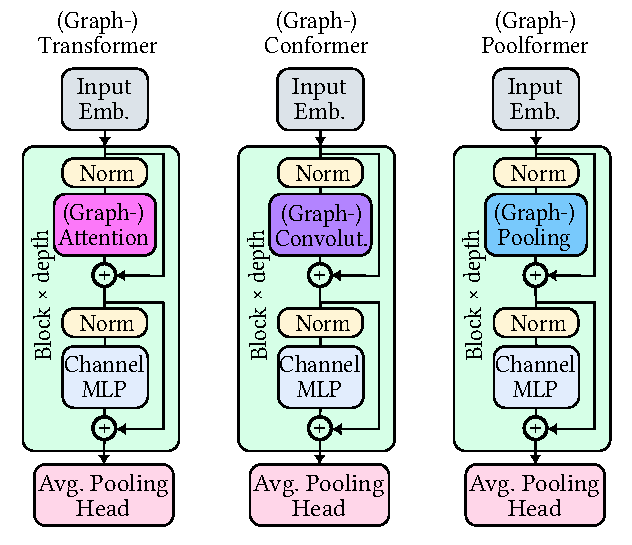
\includegraphics[width=0.7\textwidth]{./architectures/theory/metaformer/token-mixer-lineup.pdf}}
    \caption{Different possible instances of the metaformer architecture presented in \autoref{fig:metaformer-architecture}.
        All structural elements are equivalent to the respective ones in that figure. 
        Only for the placeholder \emph{token mixer}, an \emph{attention-}, \emph{convolution-} and \emph{pooling-}module were inserted, to respectively generate a \emph{transformer}, \emph{conformer} and \emph{poolformer}.
        As different types of convolutions can be defined, the shown models are still technically \emph{classes} of models, but the figure should be enough to convey the concept of token mixer swapping.
        It is important to understand, that the different models' \emph{only difference} is the token mixer they are using.
        The graph versions of the operations are discussed in \autoref{sec:architectures-graphs}.
    }
    \label{fig:token-mixer-lineup}
\end{figure}

The name of the metaformer results from the name of the used token mixer.
A overview is given in \autoref{table:metaformer-names}

\begin{table}[htbp]
    \centering
    \makebox[\textwidth][c]{
        \begin{tabular}{llll} 
            \toprule
            Token mixer & Name & Short & Strict\\  
            \midrule 
            sdp attention & (Vision-)Transformer & TF & yes\\
            attention, masked to nn & Graph (Vision-)Transformer NN & GTF-NN & yes\\
            attention, masked to nnn & Graph (Vision-)Transformer NNN & GTF-NNN & yes\\
            pooling & Poolformer & PF & yes\\
            graph pooling, nn & Poolformer & GPF-NN & yes\\
            graph pooling, nnn & Poolformer & GPF-NNN & yes\\
            full convolution & Conformer & CF & no\\
            symm. convolution, nn & symm. Conformer NN & SCF-NN & no\\
            symm. convolution, nnn & symm. Conformer NNN & SCF-NNN & no\\
            depthw. convolution & dConformer & DCF & yes\\
            symm. depthw. convolution, nn & symm. dConformer NN & SDCF-NN & yes\\
            symm. depthw. convolution, nnn & symm. dConformer NNN & SDCF-NNN & yes\\
            depthw. graph convolution & graph dConformer & GDCF & yes\\
            symm. depthw. graph conv., nn & symm. graph dConformer NN & SGDCF-NN & yes\\
            symm. depthw. graph conv., nnn & symm. graph dConformer NNN & SGDCF-NNN & yes\\
            \bottomrule
        \end{tabular}
    }
    

    \vspace{0.5cm}
    \caption{Overview of the most important metaformer networks. If a network mixes along the \emph{embed dimension} during the token mixing, it is not deemed strict.
    For images or other data stored in rectangular tensor form, the graph- and non-graph-version of poolformer and conformer are equivalent.
    Only the graph variants use the localization bias of data that can not be canonically stored in tensor form. 
    }
    \label{table:metaformer-names}
\end{table}

The table contains an overview of all the metaformer variants that are examined in this thesis.
However other combinations are possible. \emph{GDCF}, \emph{SCF-NN} and \emph{SCF-NNN} are not implemented in the accompanying code \cite{selfPhysics, selfComputerScience}.

How the graph-equivalent modules \emph{graph (depthwise) convolution}, \emph{graph pooling} and \emph{graph masked attention} can be constructed, is described in \autoref{sec:architectures-graphs}.

An exchange of the token mixer module can have different benefits. 
Some can use specially tailored inductive biases to aid the model with its calculation.
Others vary in their storage or computational requirement.
Even more specialized architectures can be attained, if hyperparameters like the embed dimension or the choice of token mixer is varied across the depth of the metaformer. 
Starting with a poolformer of high embed dimension for the first blocks for feature extraction and then reducing the embed dimension to employ a high performance attention module for the final evaluation can result in higher performance than both of the models on their own \cite{metaformerPaper}. 
Hybrid approaches are not discussed in this paper's experiments, but could be a target for further research.

A further modification is shown in \autoref{fig:metaformer-architecture} for the last element.
An \emph{average pooling} operator is used in conjunction with a \emph{MLP} to reshape the output to dimension necessary for the task. 
In the original vision transformers, a \emph{classifier token} was used \cite{dinoPaper}, as this was motivated by the language processing origins of the transformer.
Experiments (during the writing of this thesis) have shown, that the vision transformer performed better on our use cases, if the average pooling head was used, instead of the classifier token. 
Therefore the average pooling head is included as a fixed component of the metaformer architecture in this thesis.
